\section {Oscillation systematics}
\label{sec:eval_osc_systematics}


\subsection {Inputs uncertainties for systematic error evaluation}
\label{sec:systematics_inputs}

The uncertainties considered in this analysis are summarized in Tab. \ref{tab:input_uncertainties}.
In the presence of these systematic uncertainties, Eq. \ref{eq:far_prediction_no_nd280_spectrum_final}
may be re-written as
{
\arraycolsep=2pt
\begin{equation}
\displaystyle
\begin{array}{lcl}
  N_{SK;r}^{exp} & = &
    f_{norm} \cdot f_{FSI;r} \cdot (1+\Delta{N_{SK;r}}(f_{E}^{SK})) 
      \frac{ \displaystyle N^{obs}_{ND280;CC-like} }
           { \displaystyle f_{\epsilon}^{ND280} \sum_{m\prime} N^{MC}_{ND280;m\prime} \cdot 
                \displaystyle \Big( \prod_{m_{s}} f_{R_{\sigma};m_{s}} \delta_{m\prime;m_{s}} \Big) }
    \cdot \\
    & &
    {\displaystyle
    \sum_{m,t}
        P_{m;t}^{surv} \cdot
        N_{SK;m;r;t}^{MC} \cdot
        \Big( \prod_{m_{s}} f_{R_{\sigma};m_{s}} \delta_{m;m_{s}} \Big) \cdot
        \Big( f_{\sigma_{CCQE};t} \delta_{m;CCQE} \Big) \cdot
        w^{Ch.}_{m;t}({\bf \rho^{\Phi_{SK}}})
     }
\end{array}
\label{eq:far_prediction_no_nd280_spectrum_final_with_systematics}
\end{equation}
}
As explained in Tab. \ref{tab:input_uncertainties},
the energy scale uncertainty is taken into account by scaling the reconstructed energy distribution
bin edges and, assuming uniform distribution of events within the 50 MeV bins,
calculating the number of events gained from / lost to neighbouring bins.
The term $\Delta{N_{SK;r}}$ in above equation expresses the net gain of events at the 
reconstructed energy bin $r$ as a result of SuperK energy scale variations. 
The term $f_{R_{\sigma};m_{s}}$,
where the index $m_{s}$ runs over CC1$\pi$, CCoth and NC,
denotes the MC template modification factor due to the uncertainty
on any of the cross section ratios (relative to CCQE) described in Tab. \ref{tab:input_uncertainties},
while the term $\delta_{m\prime;m}$ is 1 for $m\prime=m$ and 0 otherwise.
Finally, $w^{Ch.}_{m;t}({\bf \rho^{\Phi_{SK}}})$ denotes flux weights generated from 
the SuperK $\nu_{\mu}$ flux true energy bin-to-bin correlation matrix ${\bf \rho^{\Phi_{SK}}}$
using the Cholesky method (see Sec. \ref{sec:cholesky}). 
These weights (ratios of tweaked over nominal 2010d(v2) $\nu_{\mu}$ neutrino fluxes)
are applied only to the $\nu_{\mu}$ SuperK MC templates
and depend on the true energy bin t. 
The weights are constructed so that they have no effect on the 
integrated number of SuperK 1-ring $\mu$-like events.
All other factors appearing in Eq. \ref{eq:far_prediction_no_nd280_spectrum_final_with_systematics} 
are explained in Tab. \ref{tab:input_uncertainties}.

%
% Table with systematic parameters
%

\begin{table*}[htb]
\center
\renewcommand{\arraystretch}{1.75} % enlarge line spacing
\begin{tabular}{p{0.12\textwidth}p{0.88\textwidth}}
%
% SuperK
%
\hline
\multicolumn {2}{l} { {\bf SuperK detector uncertainties} } \\
\hline
\parbox{0.12\textwidth}
{
   $f_{\epsilon}^{SK}$  
}&
\parbox{0.88\textwidth}
{
    \vspace{0.2cm}
    Combined efficiency uncertainty due to fiducial volume, reduction chain, 
    Outer Detector cut, ring counting and PID cut uncertainties.
    (CCQE: 7.8\%, CCnonQE: 25.5\%, NC: 115.1\%, $\nu_{e}$ CC: 100\% \cite{SuperKAnalysisInputs}).
    Applied to corresponding SuperK MC templates.\\
}\\
\parbox{0.12\textwidth}
{
   $f_{E}^{SK}$  
}&
\parbox{0.88\textwidth}
{
    \vspace{0.2cm}
    Reconstructed energy scale error (1\% \cite{SuperKAnalysisInputs}). 
    Applied to SuperK MC templates by scaling bin edges and,
    assuming uniform distribution of events within the 50 MeV bins, calculating the number of events 
    gained from / lost to neighbouring bins.\\
}\\
\hline
%
% nd280 detector systematics
%
\multicolumn {2}{l} { {\bf ND280 detector uncertainties} } \\
\hline
\parbox{0.12\textwidth}
{ 
   $f_{\epsilon}^{ND280}$  
}&
\parbox{0.88\textwidth}
{
    \vspace{0.2cm}
    Efficiency error (5\% \cite{ND280AnalysisInputs}).
    Applied to ND280 MC templates.\\
}\\
\hline
%
% Beam systematics
%
\multicolumn {2}{l} { {\bf Flux uncertainties} } \\
\hline
\parbox{0.12\textwidth}
{ 
   $f_{norm}$ 
}&
\parbox{0.88\textwidth}
{
    \vspace{0.2cm}
    Flux normalization uncertainty.
    Uncertainty, expressed relatively to the $N_{SK}/N_{ND280}$ ratio predicted by the MC,
    is calculated against oscillation and other systematic parameters 
    using code provided by the Beam WG \cite{BeamNormErrCode}.
    Calculated uncertainty for nominal MC and oscillations with parameters
    $sin^{2}2\theta_{23}$ = 1.00 and $\Delta m^{2}_{23}$ = 2.4$\times10^{-3}$ $eV^{2}/c^{4}$
    is around 6.6\%.\\
}\\
\hline
\parbox{0.12\textwidth}
{ 
    ${\bf \rho^{\Phi_{SK}}}$ 
}&
\parbox{0.88\textwidth}
{
    \vspace{0.2cm}
    Flux shape uncertainty. Expressed in terms of true energy bin-to-bin 
    correlation matrix for SuperK $\nu_{\mu}$ flux provided by the Beam WG \cite{BeamShapeErr}.
    Uncertainty is propagated using the Choleskly method (see Sec. \ref{sec:cholesky}).\\
}\\
\hline
%
% Neutrino Generator
%
\multicolumn {2}{l} { {\bf Neutrino Generator (GENIE/NEUT) model uncertainties} } \\
\hline
\parbox{0.12\textwidth}
{ 
    \vspace{0.2cm}
    $f_{\sigma_{CCQE};t}$ 
}&
\parbox{0.88\textwidth}
{
    \vspace{0.2cm}
    CCQE cross section uncertainty. It respresents only ``residual'' CCQE uncertainty not
    cancelled-out in the near to far extrapolation due to the fact that the near and far
    detectors sample different flux energy ranges and they are made of different nuclear
    targets. Therefore the uncertainty is applied to SuperK MC templates only.
    The uncertainty has true neutrino energy dependence \cite{NIWGErr}
    which is denoted here by the true neutrino energy bin number t.\\
   
}\\
\parbox{0.12\textwidth}
{ 
    \vspace{0.2cm}
    $f_{\sigma_{CC1\pi}/\sigma_{CCQE}}$ 
}&
\parbox{0.88\textwidth}
{
    \vspace{0.2cm}
    Fractional uncertainty on CC1$\pi$/CCQE cross section ratio
    (30\% for true energy below 2 GeV and 20\% for energy above 2 GeV \cite{NIWGErr}).
    Applied both to corresponding SuperK and ND280 MC templates.\\
}\\
\parbox{0.12\textwidth}
{ 
    \vspace{0.2cm}
    $f_{\sigma_{CCoth}/\sigma_{CCQE}}$ 
}&
\parbox{0.88\textwidth}
{
    \vspace{0.2cm}
    Fractional uncertainty on CCother/CCQE cross section ratio
    (30\% for true energy below 2 GeV and 25\% for energy above 2 GeV \cite{NIWGErr}).
    Applied both to corresponding SuperK and ND280 MC templates.\\ 
}\\
\parbox{0.12\textwidth}
{ 
    \vspace{0.2cm}
    $f_{\sigma_{NC}/\sigma_{CCQE}}$ 
}&
\parbox{0.88\textwidth}
{
    \vspace{0.2cm}
    Fractional uncertainty on NC/CCQE cross section ratio
    (36\% \cite{NIWGErr}).
    Applied both to corresponding SuperK and ND280 MC templates.\\   
}\\
\parbox{0.12\textwidth}
{ 
    \vspace{0.2cm}
    $f_{FSI;r}$ 
}&
\parbox{0.88\textwidth}
{
    \vspace{0.2cm}
    Uncertainty on effect of FSI (final state interaction / intranuclear hadron transport).
    The uncertainty affects mainly the SuperK exclusive CCQE-like (1 $\mu$-like ring) measurement (eg. effect 
    of pion absorption in oxygen) and not the ND280 inclusive CC measurement.
    Therefore, it is applied only to SuperK MC templates.
    The error has a reconstructed energy dependence \cite{NIWGErr}
    which is denoted here by the reconstructed neutrino energy bin number r.\\
}\\
\hline
\end{tabular}\\[2pt]
\caption{
  Inputs for $\nu_{\mu}$ disappearance systematic error evaluation.
  Each parameter $f_{P}$ is a MC template modification factor accounting for the uncertainty
  on quantity P (P may be a detector efficiency, energy scale, 
  absolute cross section, cross section ratio etc.) 
  If the relative uncerianty on P is expressed by $\frac{\delta{P}}{P}$, then 
  $f_{P} = 1 + g(\mu=0;\sigma=1) * \frac{\delta{P}}{P}$
  where $g(\mu=0;\sigma=1)$ is a gaussian error with mean 0 and standard deviation of 1.
}
\label{tab:input_uncertainties}
\end{table*}

\clearpage

\subsection {Effect of systematic uncertainties on SuperK predictions}
\label{sec:systematics_tweaked_spectra}

The effect of input systematic uncertainties on predicted number of 1 $\mu$-like ring 
events (after extrapolation) is shown for both GENIE and NEUT 
in Tab. \ref{table:dnsk_noosc} (no oscillations) and
in Tab. \ref{table:dnsk_2p4Em3_1p0} (for oscillations with parameters
$sin^{2}2\theta_{23}$ = 1.0 and $\Delta m^{2}_{23}$ = 2.4$\times10^{-3}$ $eV^{2}/c^{4}$).
The effect of systematic parameters on various SuperK and ND280 components of
the calculation as well as in the predicted 1 $\mu$-like ring event reconstructed energy
spectrum is presented in detail in Appendix \ref{appendix:effect_of_systematics}.

\begin{table*}[htb]
\center
\renewcommand{\arraystretch}{1.75} % enlarge line spacing
\begin{tabular}{|c|c|c|}
\hline
       & GENIE & NEUT \\
Error source  &
  $\delta{N^{exp}_{SK}}/N^{exp}_{SK}$  &
  $\delta{N^{exp}_{SK}}/N^{exp}_{SK}$  \\
\hline
SuperK CCQE efficiency            &   $\pm$6.4\%      &   $\pm$6.4\%      \\
SuperK CCnonQE efficiency         &   $\pm$3.9\%      &   $\pm$4.3\%      \\
SuperK NC efficiency              &   $\pm$2.6\%      &   $\pm$2.1\%      \\
SuperK $\nu_{e}$ CC efficiency    &   $\pm$0.0\%      &   $\pm$0.0\%      \\
ND280 efficiency                  &   +5.3\% -4.8\%   &   +5.3\% -4.8\%   \\
Flux normalization                &   $\pm$9.6\%      &   $\pm$9.7\%      \\
CCQE cross section                &   $\pm$4.3\%      &   $\pm$4.1\%      \\
CC1pi/CCQE cross section ratio    &   +2.7\% -2.4\%   &   +2.2\% -2.0\%   \\
CCother/CCQE cross section ratio  &   +5.9\% -5.2\%   &   +5.4\% -4.8\%   \\
NC/CCQE cross section ratio       &   $\pm$0.7\%      &   $\pm$0.8\%      \\
FSI                               &   $\pm$3.3\%      &   $\pm$3.3\%      \\
\hline
Total                             &   +16.0\% -15.5\% &   +15.7\% -15.3\% \\
\hline
\end{tabular}\\[2pt]
\caption{
  Effect of 1$\sigma$ systematic parameter variation on the non-oscillated number of 1 $\mu$-like ring events
  predicted by GENIE and NEUT (after extarpolation).
}
\label{table:dnsk_noosc}
\end{table*}


\begin{table*}[htb]
\center
\renewcommand{\arraystretch}{1.75} % enlarge line spacing
\begin{tabular}{|c|c|c|}
\hline
       & GENIE & NEUT \\
Error source  &
  $\delta{N^{exp}_{SK}}/N^{exp}_{SK}$  &
  $\delta{N^{exp}_{SK}}/N^{exp}_{SK}$  \\
\hline
SuperK CCQE efficiency            &   $\pm$4.8\%      &   $\pm$4.7\%       \\
SuperK CCnonQE efficiency         &   $\pm$7.7\%      &   $\pm$8.4\%       \\
SuperK NC efficiency              &   $\pm$9.5\%      &   $\pm$7.5\%       \\
SuperK $\nu_{e}$ CC efficiency    &   $\pm$0.1\%      &   $\pm$0.1\%       \\
ND280 efficiency                  &   +5.3\% -4.8\%   &   +5.3\% -4.8\%    \\
Flux normalization                &   $\pm$6.6\%      &   $\pm$6.3\%       \\
CCQE cross section                &   $\pm$3.0\%      &   $\pm$2.5\%       \\
CC1pi/CCQE cross section ratio    &   +0.1\% -0.2\%   &   +0.4\% -0.5\%    \\
CCother/CCQE cross section ratio  &   +5.1\% -4.5\%   &   +4.1\% -3.7\%    \\
NC/CCQE cross section ratio       &   $\pm$1.5\%      &   $\pm$0.9\%       \\
FSI                               &   $\pm$5.8\%      &   $\pm$6.0\%       \\
\hline
Total                             &   +17.8\% -17.5\% &   +16.6\% -16.3\%  \\
\hline
\end{tabular}\\[2pt]
\caption{
  Effect of 1$\sigma$ systematic parameter variation on the number of 1 $\mu$-like ring events
  predicted by GENIE and NEUT (after extarpolation) for oscillations with parameters
  $sin^{2}2\theta_{23}$ = 1.0 and $\Delta m^{2}_{23}$ = 2.4$\times10^{-3}$ $eV^{2}/c^{4}$.
}
\label{table:dnsk_2p4Em3_1p0}
\end{table*}


\begin{figure*}[htb]
\center
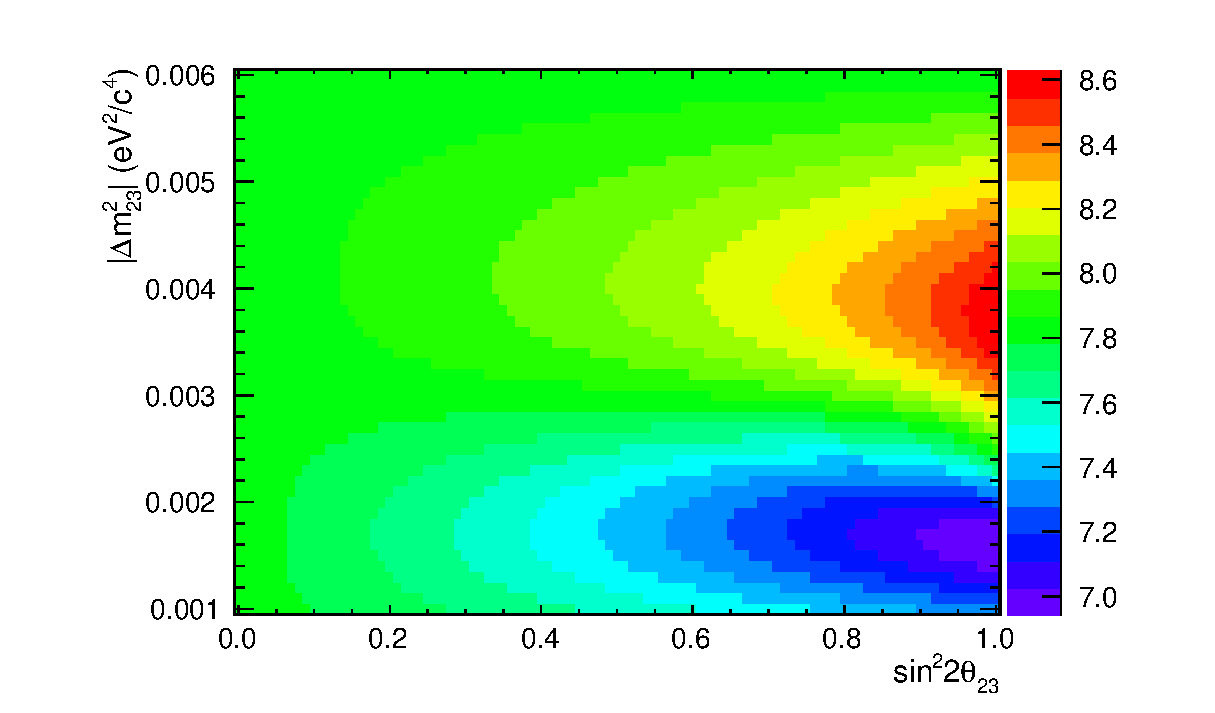
\includegraphics[width=38pc]{./images/predicted_spectrum/systematic_variations/frac_nsk_err_twk_xsec.eps}
\caption{
  Percentage uncertainty
  on expected numbers of 1-ring $\mu$-like events (after extrapolation)
  in the 0-10 GeV reconstructed energy range
  due to quoted cross uncertainties only.
  Over the oscillation parameter space considered by this analysis, 
  the uncertainty in the 7\% to 8.6\% range.
  This plot can be directtly compared 
  with the GENIE-NEUT difference shown in Fig. \ref{fig:genie_neut_nsk_difference_osc_param_grid}.
}
\label{fig:nsk_uncertainty_osc_param_grid_xsec_err_only}
\end{figure*}
  

\subsection {Evaluating systematics at oscillation best-fit point}
\label{sec:systematics_at_osc_bestfit}

Systematics, at a given point of the oscillation parameter space, are calculated by 
fitting a large number (typically 10,000) of toy experiments, generated with the 
given oscillation parameters and with randomly varied systematic parameters.
The systematic error on $sin^{2}2\theta_{23}$ and $\Delta m^{2}_{23}$ 
are taken to be the one standard deviation of the corresponding best-fit parameter distribution.
In order to decouple statistical and systematic effects, 
no statistical fluctuations are included in the toy experiments.
The effect of each systematic parameter is calculated separately
and then they are combined by adding them in quadratures.
An evaluation of the 3.23$\times 10^{19}$-POT T2K disapearance analysis systematics for 
oscillation parameters near the MINOS best fit point 
($sin^{2}2\theta_{23}$ = 0.9 and $\Delta m^{2}_{23}$ = 2.4$\times10^{-3}$ $eV^{2}/c^{4}$)
is shown in Tab. \ref{table:systamatics_at_2p4Em3_0p9}.

\begin{table*}[htb]
\center
\renewcommand{\arraystretch}{1.75} % enlarge line spacing
\begin{tabular}{|c|cc|cc|}
\hline
              &
  \multicolumn{2}{c|} { GENIE } &
  \multicolumn{2}{c|} { NEUT  } \\
Error source  &
  $\Big(\frac{\delta{\Delta m^{2}_{23}}}{\Delta m^{2}_{23}}\Big)$  & $\Big(\frac{\delta{\sin^{2}2\theta_{23}}}{sin^{2}2\theta_{23}}\Big)$  &
  $\Big(\frac{\delta{\Delta m^{2}_{23}}}{\Delta m^{2}_{23}}\Big)$  & $\Big(\frac{\delta{\sin^{2}2\theta_{23}}}{sin^{2}2\theta_{23}}\Big)$  \\
\hline
SuperK CCQE efficiency            &   0.3\%   &   1.7\%      &   0.5\%   &   1.6\%  \\
SuperK CCnonQE efficiency         &   0.5\%   &   1.1\%      &   0.5\%   &   1.3\%  \\
SuperK NC efficiency              &   3.9\%   &   3.1\%      &   3.5\%   &   3.0\%  \\
SuperK $\nu_{e}$ CC efficiency    &   0.0\%   &   0.0\%      &   0.0\%   &   0.0\%  \\
SuperK energy scale               &   0.3\%   &   0.2\%      &   0.5\%   &   0.2\%  \\
ND280 efficiency                  &   0.1\%   &   1.5\%      &   0.3\%   &   1.4\%  \\
Flux normalization                &   0.1\%   &   1.6\%      &   0.3\%   &   1.5\%  \\
Flux shape                        &   2.3\%   &   0.5\%      &   2.2\%   &   0.6\%  \\
CCQE cross section                &   1.2\%   &   1.5\%      &   1.0\%   &   1.5\%  \\
CC1pi/CCQE cross section ratio    &   0.2\%   &   0.6\%      &   0.1\%   &   0.3\%  \\
CCother/CCQE cross section ratio  &   0.1\%   &   1.7\%      &   0.1\%   &   1.5\%  \\
NC/CCQE cross section ratio       &   1.2\%   &   0.5\%      &   1.2\%   &   0.5\%  \\
FSI                               &   0.1\%   &   0.7\%      &   0.3\%   &   0.6\%  \\
\hline
Total                             &   5.1\%   &   5.3\%      &   4.7\%   &   5.0\%  \\
\hline
\end{tabular}\\[2pt]
\caption{
  Oscillation systematics evaluated at
  $sin^{2}2\theta_{23}$ = 0.9 and $\Delta m^{2}_{23}$ = 2.4$\times10^{-3}$ $eV^{2}/c^{4}$.
}
\label{table:systamatics_at_2p4Em3_0p9}
\end{table*}


\subsection {Including systematics in calculation of confidence regions}

In the context of the Feldman-Cousins analysis, systematic errors are naturally included in
the confidence regions by including systematic variations in the toy experiments used for
calculating the $\Delta\chi^{2}_{a}$ surfaces (where $a$ denotes the specified confidence level)
as a function of $sin^{2}2\theta_{23}$ and $\Delta m^{2}_{23}$. 
The procedure was outlined in Sec. \ref{sec:contour_fc}.

\subsection {Handling correlated systematics: Cholesky decomposition method}
\label{sec:cholesky}

The LU decomposition is a well-known factorization of a matrix ${\bf C}$
as a product of a lower triangular matrix ${\bf L}$ and an upper triangular matrix ${\bf U}$.
The LU decomposition has several applications in scientific computing \cite{NumRecipCholesky}.
Let ${\bf C}$ be a square, symmetric, positive-definite\footnote{
  ${\bf v} \cdot {\bf C} \cdot {\bf v} > 0$ for every vector ${\bf v}$.} matrix.
Under the stated conditions, there exists a special factorization of ${\bf C}$, the Cholesky decomposition,
which is significantly {\em more efficient} than the generic LU decomposition.
Rather than factorizing ${\bf C}$ as the product of two independent matrices ${\bf L}$ and ${\bf U}$,
the Cholesky method factorizes ${\bf C}$ as the product 
of a lower triangular matrix ${\bf L}$ and its transpose matrix:
\begin{equation}
\displaystyle 
  {\bf C} = {\bf L} \cdot {\bf L}^{T} 
\end{equation}
The Cholesky decomposition algorithm can be found in \cite{NumRecipCholesky}.

The Cholesky decomposition is commonly used for Monte Carlo simulation of systems with correlated variables.
Let $S_{N}$ be such a system whose dimensionality is $N$
and let ${\bf C}$ be the $N \times N$ matrix which describes the covariance of the 
$N$ simulated variables.
The covariance matrix ${\bf C}$ is decomposed to obtain the lower triangular matrix ${\bf L}$.
Let ${\bf u}$ be a $N$-dimensional vector of uncorrelated variables;
each vector element $u_{i}$ can be randomly generated from a gaussian
distribution with a mean of 0 and a standard deviation of 1.
The vector
\begin{equation}
\displaystyle 
  {\bf x} = {\bf L} \cdot {\bf u}
\end{equation}
has the covariance properties of $S_{N}$.


